% !TEX program = xelatex
\DocumentMetadata{lang=en} % required for transparent package
\documentclass[11pt,aspectratio=169]{beamer}

% remove footcite numbers
\makeatletter
\def\@makefnmark{}
\makeatletter

\setbeamersize{text margin left=5mm,text margin right=5mm} 

\newcommand\focus[1]{%
	{\alert{\textbf{#1}}}%
}

\usepackage{amsthm,amsmath,amssymb,braket,fontspec,unicode-math,fontenc,transparent}
\usepackage[absolute,overlay]{textpos}

\usetheme{moloch}
\setmainfont{Linux Libertine}
\setsansfont{Linux Libertine}
\setmathfont{Fira Math}
\setmathfont{latinmodern-math.otf}[range={frak,\bigcap,\bigcup}]

\usepackage[backend=bibtex,url=false,doi=false,style=authoryear]{biblatex}
\setbeamertemplate{bibliography item}{}
\bibliography{bib}
\AtBeginBibliography{\scriptsize}

\graphicspath{{./figures/}}

\setbeamerfont{title}{size=\LARGE\scshape}
\setbeamerfont{author}{size=\large}
\setbeamerfont{institute}{size=\large}
\setbeamerfont{date}{size=\large}
\setbeamerfont{frametitle}{size=\large\scshape}
\setbeamerfont{sectiontitle}{size=\small\scshape}

\title{Research Progress Report: 2024 - 2025}
\author{\bf Abhirup Mukherjee}
\institute{
Department of Physical Sciences, IISER Kolkata, Mohanpur}
\date{July 25, 2025}

\begin{document}

\centering

\begin{frame}
\maketitle

\begin{textblock*}{0.3\textwidth}(5cm, 6.5cm)
	\includegraphics[width=0.4\textwidth]{epqm_logo_mod.jpeg}
	\hspace*{\fill}
	\includegraphics[width=0.4\textwidth]{dps_logo.jpeg}
\end{textblock*}
\hspace*{\fill}
\end{frame}

\begin{frame}{Acknowledgements}
	\flushleft
	\hspace*{20pt}
	\focus{Collaborators}: Debraj, Arnabesh, Sukalyan, Prof. S. R. Hassan, Prof. Anamitra Mukherjee, Prof. N S Vidhyadhiraja, Prof. A Taraphder\\
	\hspace*{20pt}
	\focus{Funding agencies}: IISER Kolkata, SERB
	\vspace*{\fill}

	\hspace*{\fill}
	\includegraphics[width=0.1\textwidth]{SERB.png}
	\hspace*{\fill}
	\includegraphics[width=0.1\textwidth]{dps_logo.jpeg}
	\hspace*{\fill}
	\includegraphics[width=0.1\textwidth]{epqm_logo_mod.jpeg}
	\hspace*{\fill}
\end{frame}

\begin{frame}{Publications and Ongoing Projects}
\focus{Published}

\begin{minipage}{0.49\textwidth}
\begin{itemize}
	\item 2023 New J. Phys. 25 113011
	\item 2024 J. Phys. A: Math. Theor. 57 275401
\end{itemize}
\end{minipage}
\begin{minipage}{0.49\textwidth}
\begin{itemize}
	\item \transparent{0.4}{2022 Phys. Rev. B 105, 085119}
	\item \transparent{0.4}{2023 J. Phys.: Condens. Matter 35 315601}
\end{itemize}
\end{minipage}

\vspace*{\fill}

\focus{Currently in Progress}

\begin{minipage}{0.49\textwidth}
\begin{itemize}
	\item Development of auxiliary model-based method for interacting electrons [{\bf arXiv}:2507.17201].
\end{itemize}
\end{minipage}
\begin{minipage}{0.49\textwidth}
\begin{itemize}
	\item Studies of plateau-to-plateau transition in integer quantum hall systems.
\end{itemize}
\end{minipage}

\vspace*{\fill}

\focus{Ongoing Collaborations}

\begin{minipage}{0.49\textwidth}
\begin{itemize}
	\item Breakdown of Kondo screening in presence of magnetic field [DD, {\bf AM}, SL]
	\item Quantum critical Mott MIT in 3-orbital impurity model [AK, DD, {\bf AM}, NSV, SL]
	\item Universal features of Kondo breakdown in impurity models [DD, {\bf AM}, SL]
\end{itemize}
\end{minipage}
\begin{minipage}{0.49\textwidth}
\begin{itemize}
	\item Search for non-Fermi liquid physics in mixed-valence eSIAM [AS, {\bf AM}, SL]
	\item Spin-liquid and non-Fermi liquid phases in frustrated systems [SD, {\bf AM}, SL]
	\item Hawking-Page entanglement transition in a Kondo system [DD, {\bf AM}, SL]
\end{itemize}
\end{minipage}
\end{frame}

\section{Ongoing Collaborations}

\begin{frame}{Hawking-Page Entanglement Transition in a Kondo System}
\footcite{Hawking1974,Hawking1975,Page1993}
Hawking radiation + black hole evaporation appears to \focus{violate unitarity}
\begin{itemize}
	\item Initially system is in \focus{pure state}.
	\item Hawking's calculation: increasing entanglement between radiation and interior
	\item This leads to \focus{mixed state} at \(t=\infty\), but mixedness cannot change under \focus{unitary evolution}.
\end{itemize}


\begin{minipage}{0.45\textwidth}
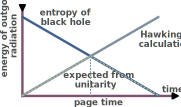
\includegraphics[width=\textwidth]{hawking-page.pdf}
\end{minipage}
\begin{minipage}{0.5\textwidth}
	\begin{itemize}
		\item Unitarity means entanglement of radiation \focus{must decrease} after page time.
		\item Can we replicate this behaviour in a \focus{quantum system}?
	\end{itemize}
	
\end{minipage}

\end{frame}

\begin{frame}{Hawking-Page Entanglement Transition in a Kondo System}
\flushleft
(D Debata, {\bf A Mukherjee}, S Lal)\\[10pt]
Consider a \focus{two-impurity model} (\(d\), \(d^\prime\)), with spin-exchange interaction between the impurities
\begin{minipage}{0.5\textwidth}
\begin{itemize}
	\item \(d^\prime (d) \to\) black hole interior (boundary)
	\item \(0 \to\) radiation outside the black hole
\end{itemize}
\vspace{10pt}
	
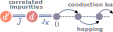
\includegraphics[width=\textwidth]{blackHoleModel.pdf}
\end{minipage}
\begin{minipage}{0.45\textwidth}
\includegraphics[width=\textwidth]{blackhole.pdf}
\end{minipage}

Mutual-information between \(d^\prime\) and \(0\) shows behaviour similar to Page curve.

\end{frame}

\begin{frame}{Universal Features of Kondo Breakdown in Impurity Models}
\footcite{fabrizio2017kondo,RADEMAKER2025}
\focus{Kondo screening} (or its breakdown) lies at the heart of emergence in interacting electrons.

\vspace{\fill}
\vspace{\fill}
\begin{minipage}{0.48\textwidth}
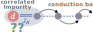
\includegraphics[width=\textwidth]{kondo.pdf}
\end{minipage}
\hspace{\fill}
\begin{minipage}{0.48\textwidth}
\focus{What is screening?} \\
Whether the impurity spin forms a correlated \focus{non-magnetic state} with local spin density of conduction electrons, at low temperature
\end{minipage}
\vspace{\fill}

\begin{itemize}
	\item SCREENING \(\to\) gapless \focus{1-particle} excitations
	\item ABSENCE of screening \(\to\) excitations are \focus{gapped}
	\item PARTIAL breakdown \(\to\) excitations are \focus{exotic}
\end{itemize}
\vspace{\fill}

Obtaining a broader understanding of features of partial screening is important, particularly since such states appear near \focus{critical points}!

\end{frame}

\begin{frame}{Universal Features of Kondo Breakdown in Impurity Models}
\footcite{Mukherjee_2023,Patra_2023}
\flushleft
\vspace{-20pt}
(D Debata, {\bf A Mukherjee}, S Lal)\\[5pt]
We are studying two models that display partial breakdown of Kondo screening:
\begin{itemize}
	\item eSIAM: Kondo breakdown through charge fluctuations in the bath
	\item two-channel Kondo model: Kondo breakdown due to competing screening tendencies
\end{itemize}
\vspace{10pt}

\begin{minipage}{0.45\textwidth}
\includegraphics[width=\textwidth]{intra.pdf}
\end{minipage}
\begin{minipage}{0.5\textwidth}
\begin{itemize}
	\item Universal signatures of Kondo breakdown include \focus{partial magnetisation}, partial phase shift.
	\item More recently, we are looking into \focus{long-range entanglement} and correlations near Kondo breakdown.
\end{itemize}
\end{minipage}
\end{frame}
	
\section{A New Auxiliary Model Approach to Systems of Interacting Electrons \\ \small{({\it A Mukherjee}, S R Hassan, Anamitra Mukherjee, N S Vidhyadhiraja, A Taraphder, S Lal. arXiv:2507.17201)}}

\begin{frame}{Broad Objectives}
	\footcite{keimer2015quantum,Sebastian2014,Norman1998}

	\vspace*{-20pt}
\begin{itemize}
	\item[✔] Designing a \focus{new method} by which to leverage quantum impurity models towards understanding phase transitions in correlated electrons in low dimensions\\[10pt]
	\item[✔] Study the highly non-trivial Mott MIT through the \focus{pseudogap} in the context of the cuprates \\[10pt]
	\item[✔] Characterise the \focus{parent metal} that gives way to an interacting Mott insulator.
\end{itemize}

\hspace*{\fill}
\includegraphics[width=0.3\textwidth]{cupratesDiagram.png}
\hspace*{\fill}
\includegraphics[width=0.25\textwidth]{fermiArc.png}
\hspace*{\fill}
\end{frame}

\begin{frame}{Momentum-Resolved Renormalisation Group Flows}
\begin{minipage}{0.19\textwidth}
	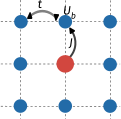
\includegraphics[width=\textwidth]{pWaveEsiam.pdf}
\end{minipage}
\begin{minipage}{0.45\textwidth}
	Hamiltonian RG equations of \\
	\focus{embedded e-SIAM}
	\[\Delta J^{(j)}_{{\bf k}_1, {\bf k}_2} = -\sum_{{\bf q} \in \text{PS}} \frac{J^{(j)}_{{\bf k}_2,{\bf q}} J^{(j)}_{{\bf q},{\bf k}_1} + 4J^{(j)}_{{\bf q}, {\bf \bar q}} W_{{\bf \bar q}, {\bf k}_2, {\bf k}_1, {\bf q}}}{\omega - \frac{1}{2}|\varepsilon_j| + J^{(j)}_{{\bf q}}/4 + W_{{\bf q}}/2}\]
\end{minipage}
\begin{minipage}{0.34\textwidth}
	\includegraphics[width=\textwidth]{phaseDiagram-77-0.001.pdf}
\end{minipage}

\vspace*{\fill}
\includegraphics[width=0.32\textwidth]{SF-1.pdf}
\includegraphics[width=0.32\textwidth]{SF-3.pdf}
\includegraphics[width=0.32\textwidth]{SF-4.pdf}
	
\end{frame}

\begin{frame}{`Periodising' the Hamiltonian and Eigenstates}
	\footnote{Image: Mayank Shreshtha}
	\vspace{-20pt}
	\flushleft
	Periodising the Hamiltonian creates an \focus{extended-Hubbard} model:
	\vspace{\fill}
	\begin{minipage}{0.55\textwidth}
	\[\mathcal{H}_\text{tiled} = \sum_{{\bf r}}T^\dagger({\bf r} - {\bf r}_d)\mathcal{H}_\text{aux}({\bf r}_d)T({\bf r} - {\bf r}_d)\]
	Wavefunctions can be related using a many-body \focus{Bloch's theorem}:
	\[\ket{\Psi_\text{gs}} = \frac{1}{\sqrt N}\sum_{{\bf r}_d} e^{i {\bf k}\cdot{\bf r}_d} \ket{\psi_\text{gs}\left({\bf r}_d\right)}\]
	\vspace{-10pt}
	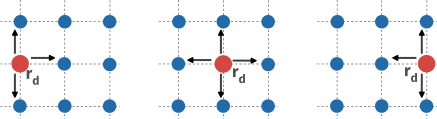
\includegraphics[width=\textwidth]{periodisation.pdf}
	\end{minipage}
	\hspace{\fill}
	\begin{minipage}{0.4\textwidth}
	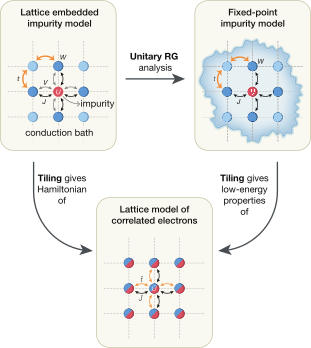
\includegraphics[width=\textwidth]{method.pdf}
	\end{minipage}

	
\end{frame}

\begin{frame}{Periodising the Greens Functions}
	\footcite{kotliar2000,verret2022}
	\begin{minipage}{0.4\textwidth}
	Greens function = \\
	sum of 1-particle \focus{\(k-\)space} Greens functions starting from \focus{all sites} in impurity model.
	\end{minipage}
	\hspace{\fill}
	\begin{minipage}{0.54\textwidth}
	\begin{equation*}\begin{aligned}
		\tilde G({\bf r}; \tilde\omega) = \frac{1}{N}\sum_{{\bf k},{\bf r}_x} \left[e^{i \left({\bf k}- {\bf k}_0\right)\cdot\left({\bf r} - {\bf r}_x\right)}G_p\left({\bf r}_x;\omega + \varepsilon_{\bf k}\right) \right. \\
	\left. + e^{-i \left({\bf k}- {\bf k}_0\right)\cdot\left({\bf r} - {\bf r}_x\right)}G_h\left({\bf r}_x;\omega - \varepsilon_{\bf k}\right)\right]
	\end{aligned}\end{equation*}
	\end{minipage}

	\vspace*{\fill}
	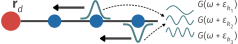
\includegraphics[width=0.8\textwidth]{greensFunc.pdf}

	\vspace*{\fill}
	\begin{minipage}{0.45\textwidth}
	Subsequently allows periodising spectral \\ 
	functions and self-energies
	\end{minipage}
	\hspace{\fill}
	\begin{minipage}{0.5\textwidth}
	\(\tilde A({\bf K}; \omega )= -\frac{1}{\pi}\text{Im}\left[\tilde G({\bf K}; \tilde\omega)\right]\)\\
	\(\tilde \Sigma({\bf K}; \omega) = \left(\tilde G^{(0)}({\bf K}; \tilde\omega)\right)^{-1} - \left(\tilde G({\bf K}; \tilde\omega)\right)^{-1}\)
	\end{minipage}
	
\end{frame}

\begin{frame}{Characterising Low-energy Excitations of the Pseudogap}
\footcite{Baskaran1991,Hatsugai1992,lanave2025}
\vspace{-20pt}

\begin{minipage}{0.6\textwidth}
\begin{itemize}
	\item Impurity spectral function shows \focus{pseudogap} (loss of central peak)
	\item Tiled \(k-\)space DOS shows \focus{partial gapping} around antinodes
	\item Self-energy shows \focus{anomalous exponent} throughout the phase
\end{itemize}
\end{minipage}
\hspace{\fill}
\begin{minipage}{0.35\textwidth}
	\includegraphics[width=\textwidth]{phaseDiagram-77-0.001.pdf}
\end{minipage}

\hspace{-8pt}
\includegraphics[width=0.29\textwidth]{kspaceDOS-77.pdf}
\includegraphics[width=0.32\textwidth]{Ad_zoomin_77-1500.pdf}
\includegraphics[width=0.39\textwidth]{selfEnergy_d_fit_77-1500.pdf}

\end{frame}

\begin{frame}{Theory for the Nodal Non-Fermi Liquid}
\begin{minipage}{0.65\textwidth}
	Exactly solvable model emerges at the \focus{critical point}.
	\[\Delta \tilde H_{{\bf q}_1 = {\bf q}_2} = \sum_{{\bf q},\sigma}\epsilon_{{\bf q}}{n}_{{\bf q},\sigma} + u\sum_{{\bf q}, \sigma}n_{{\bf q} \sigma} n_{{\bf q} \bar\sigma}\]
	\begin{itemize}
		\item Diverging self-energy at zero energy: \(\Sigma^{\prime\prime} \sim 1/\omega\)
		\item Holon-doublon deconfining excitations
	\end{itemize}
\end{minipage}
\begin{minipage}{0.3\textwidth}
\includegraphics[width=\textwidth]{SF-4.pdf}
\end{minipage}
\vspace{\fill}

\begin{minipage}{0.5\textwidth}
Greens function shows bifurcation: 
\[G = \frac{1}{2}\left[\frac{1}{\omega - u} + \frac{1}{\omega + u}\right]\]
\(\to\) \(\mathbb{Z}_2-\)symmetry breaking\\
\(\to\) change in analytic structure of self-energy
\end{minipage}
\begin{minipage}{0.45\textwidth}
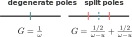
\includegraphics[width=\textwidth]{Z2.pdf}
\end{minipage}
	
\end{frame}

\begin{frame}{`Un-Fermi' Liquid Nature of the Pseudogap}
\footcite{Georgi2007,PhillipsLectures2014,Hauke2016}
Characteristics of the `\focus{Mott metal}'
\begin{itemize}
	\item low-energy excitations \focus{cannot be described} by effectively one-particle excitations (vanishing \(Z\))
	\item \focus{long-range} correlations present in the pseudogap (quantum critical matter)
	\item entanglement is \focus{multipartite} (Quantum Fisher information > 4 )
\end{itemize}
	

\includegraphics[width=0.32\textwidth]{QPR_77-1500.pdf}
\includegraphics[width=0.32\textwidth]{SF-di_77-700.pdf}
\includegraphics[width=0.32\textwidth]{qfi_77-2000.pdf}
	
\end{frame}

\begin{frame}{The Big Picture}
\footnote{Image: Mayank Shreshtha}

\vspace{-10pt}
\hspace{-10pt}
\begin{minipage}{0.4\textwidth}
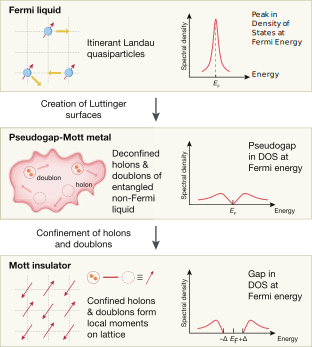
\includegraphics[width=\textwidth]{results.pdf}
\end{minipage}
\hspace{\fill}
\begin{minipage}{0.59\textwidth}
Paradigm of \focus{spontaneous symmetry breaking}
\begin{itemize}
	\item by non-zero local \focus{order parameter}
	\item \focus{short-range} entanglement and correlations
	\item excitations are \focus{one-particle} in nature (single electrons or single bosons)
	\item superconductivity, antiferromagnetism
\end{itemize}
Paradigm of \focus{fermionic criticality}
\begin{itemize}
	\item no SSB, \focus{analytic properties} of self-energy dictate phases
	\item excitations can be \focus{many-particle} in nature
	\item non-trivial entanglement (\focus{long-range}/topological)
	\item Examples: Mott metal-to-Mott insulator
\end{itemize}

\end{minipage}

\end{frame}


\section{Future Plans}

\begin{frame}{Future Plans}
	\begin{itemize}
		\item Study heavy-fermion physics using auxiliary model approach.
		\item Start consolidating results in the form of a thesis.
	\end{itemize}

	\vspace*{\fill}

	\hrule

	\vspace*{\fill}
	\Large{\bf Thank You!}
\end{frame}

\end{document}
